\documentclass[11pt,a4paper]{article}
\usepackage[margin=0.75in]{geometry}
\usepackage{graphicx}
\usepackage{authblk}
\usepackage{subcaption}
\usepackage{tikz}
\usepackage{amsmath}
\usepackage{amssymb}
\usepackage{hyperref}

\usetikzlibrary{positioning,arrows.meta}

\author[1]{Santiago Acosta\thanks{santiago\_acosta@ucsb.edu}}
\author[1]{Jonathan Skaza\thanks{skaza@ucsb.edu\\Code available at: \texttt{https://github.com/jskaza/Neural-Population-Geometry}}}
\affil[1]{Dynamical Neuroscience Graduate Program, University of California, Santa Barbara}
\title {Neural Population Geometry \\[1ex] \large ME 225NN, Winter 2025}
\date{}

\begin{document}
\maketitle
\section{Introduction}

\subsection{Problem description \& motivation}
Experimental neuroscience has seen rapid advances in recording techniques, enabling simultaneous recordings from thousands of neurons (and potentially up to a million~\cite{demas2021high}). These technological breakthroughs have driven theoretical neuroscientists to develop new methodologies for analyzing neural populations. Such large-scale analyses face distinct challenges: neurons typically respond to multiple variables simultaneously, complicating functional interpretation, while real-world tasks require robustness to complex variability that traditional tuning-based approaches struggle to capture.

In consideration of these factors, the focus of neural population analysis has transitioned from single-neuron tuning to geometric approaches that consider population-level representations~\cite{yuste2015neuron, saxena2019towards}. Traditional single-neuron tuning approaches characterize individual neurons by their response profiles to specific stimuli or task variables. For example, in the visual cortex, neurons might be classified by their preferred orientation, spatial frequency, or direction of motion, while in the motor cortex, neurons might be described by their correlation with movement direction or force. This approach, pioneered by Hubel and Wiesel's work on the visual cortex~\cite{hubel1959receptive}, has been instrumental in mapping functional properties across brain regions but struggles to capture the complex, multi-dimensional nature of neural responses during naturalistic behaviors.

The rationale behind the shift to population-level analysis is that neural computations emerge from structured, high-dimensional activity patterns rather than isolated responses of individual neurons. These patterns are conceptualized as \textit{neural manifolds}---low-dimensional geometric structures embedded in high-dimensional neural state space. The geometric properties of these manifolds---dimensionality, curvature, separability, and capacity (the number of distinct manifolds a neural system can support)---reveal computational principles governing neuronal networks~\cite{chung2021neural}. 

Neural manifolds link geometric structures to specific behavioral or cognitive variables. For example, ring-shaped manifolds have been observed in the mammalian hippocampal formation encoding head direction~\cite{chaudhuri2019intrinsic}, while grid cells conform a torus in entorhinal cortex \cite{gardner2022toroidal}. These mappings reveal how neural populations encode behaviorally relevant information and predict underlying circuitry, as confirmed by the ring-shaped wiring of fruit fly head direction circuits \cite{kim2017ring}.

This report examines the application of geometric techniques to analyze large neuronal populations—a field known as \textit{neural population geometry}. This framework provides a unified approach for understanding both biological neural circuits and artificial neural networks (ANNs). By conceptualizing neural computation as geometric transformations, we can analyze how population-level representations enable robust, efficient, and scalable information processing across biological and artificial systems. This parallel analysis reveals fundamental computational principles that transcend the specific implementation details of different neural architectures.

\subsection{Literature review}

The study of neural population geometry has emerged at the intersection of neuroscience, machine learning, and computational topology. Early work demonstrated that dimensionality reduction techniques could reveal latent structure in neural population activity, providing insights into low-dimensional dynamics underlying behavior~\cite{cunningham2014dimensionality}. This led to the discovery that neural activity during movement resides on structured manifolds shaped by motor control principles~\cite{gallego2017neural}.

Beyond low-dimensional embeddings, recent research has emphasized the topological properties of neural representations. For example, grid cell activity in the entorhinal cortex forms toroidal manifolds, capturing the periodicity of spatial coding~\cite{gardner2022toroidal}. Similarly, circular variables such as orientation and head direction exhibit ring-like manifolds, highlighting intrinsic topological structure in neural data~\cite{chaudhuri2019intrinsic}.

Parallel efforts in artificial systems have leveraged geometric frameworks to compare neural representations across biological and deep networks. These studies suggest that both systems optimize for efficient, low-dimensional embeddings that reflect task-relevant transformations~\cite{chung2021neural}. Such findings point to shared geometric principles underlying neural computation.

\subsection{Summary}
In this paper, we demonstrate how neural population geometry provides a unified framework for understanding information encoding in both biological and artificial neural systems. We focus specifically on the representation of circular variables---a fundamental computational challenge that requires preserving topological structure. Through parallel analyses of orientation encoding in the mouse visual cortex and a trained convolutional neural network (CNN), we show how similar ring-shaped manifolds emerge in both systems despite their different implementations.

Our analysis reveals that these circular manifolds arise naturally from the computational demands of the task rather than from specific architectural constraints. In the mouse visual cortex, we characterize how populations of neurons collectively form a ring-shaped manifold that encodes orientation information, with the manifold's geometry reflecting the circular topology of orientation space. Similarly, in our CNN simulation, we demonstrate how the network spontaneously develops a circular representation in its latent space when trained to discriminate orientation angles.

By comparing the geometric properties of these representations---including dimensionality, curvature, and topological structure---we identify common principles that govern how neural systems, both biological and artificial, efficiently encode circular variables. This comparative approach highlights how neural population geometry can be applied to both neuroscience and machine learning, offering insights into fundamental computational strategies that transcend specific neural implementations.

\section{Preliminaries}

\subsection{Mathematical foundations of neural manifolds}

In mathematics, a \textit{manifold} is a topological space that locally resembles Euclidean space. Formally, an $m$-dimensional manifold $\mathcal{M}$ is a topological space where each point $p \in \mathcal{M}$ has a neighborhood $U$ that is homeomorphic to an open subset of $\mathbb{R}^m$. 

In neuroscience, the concept of a \textit{neural manifold} extends this mathematical definition to describe geometric structures in neural population activity (Fig.~\ref{fig:manifolds}). Consider a population of $n$ neurons, where the activity of each neuron can be represented as a coordinate in an $n$-dimensional neural state space $\mathbb{R}^n$. Let $\mathbf{r} = (r_1, r_2, \ldots, r_n) \in \mathbb{R}^n$ represent the firing rates of these neurons at a given time. The neural manifold hypothesis posits that, during specific task execution, these population activity patterns do not explore the entire $n$-dimensional space but instead are constrained to a lower-dimensional subspace or manifold $\mathcal{M} \subset \mathbb{R}^n$, where typically $\dim(\mathcal{M}) \ll n$.

\begin{figure}
    \centering
    \includegraphics[width=0.75\linewidth]{figs/manifold_schematic.png}
    \caption{A neural manifold is formed by plotting neural activity (e.g., firing rate) in state space, where each axis is a single neuron. Note that the repeated presentation of the same stimulus does not lead to the occupancy of an identical point within the state space. Rather, neuronal variability induces fluctuations in the points derived from different trials. Consequently, each stimulus is associated not with a single point but with a point cloud, the dimensions and configuration of which are contingent upon the magnitude and nature of the neuronal variability. One may be interested in the manifold that emerges in response to a particular stimulus or whether there is separability among manifolds from multiple stimuli. Figure from \cite{Perich2024}.}
    \label{fig:manifolds}
\end{figure}

Formally, we can define a neural manifold as follows: Let $\mathbf{r}(t) \in \mathbb{R}^n$ represent the population activity at time $t$. For a given task or stimulus condition $s$ from a set of possible conditions $\mathcal{S}$, the neural manifold $\mathcal{M}_s$ is defined as:

\begin{equation}
\mathcal{M}_s = \{\mathbf{r}(t) \in \mathbb{R}^n : \text{condition } s \text{ is presented at time } t\}
\end{equation}

It is important to note that real neural data exhibits characteristics that extend beyond the strict mathematical definition of a manifold in two key ways:

\begin{enumerate}
    \item \textit{Neural variability}: When the same stimulus is presented repeatedly, neural responses vary due to stochastic processes in neural firing. This variability is thought to be fundamental to neural coding and transforms what would be a sparse set of isolated points (one per stimulus) into richer \textit{point clouds} (clusters of points for each stimulus). These point clouds collectively define the empirical neural manifold, with the distribution and statistical properties of responses containing potentially important information about the neural code.
    
    \item \textit{Sparse sampling}: Experimental limitations often allow only a finite sampling of possible stimuli or conditions, providing discrete observations of what is theoretically a continuous underlying manifold structure.
\end{enumerate}

\subsection{Classes of neural manifolds}

Several types of neural manifolds have been identified in neuroscience research:

\begin{enumerate}
    \item \textit{Object manifolds} or \textit{perceptual manifolds} arise in sensory neural populations as a result of identity-preserving variations in stimulus properties. For example, if $\mathbf{x} \in \mathbb{R}^d$ represents a stimulus (e.g., an image) and $T_\theta: \mathbb{R}^d \rightarrow \mathbb{R}^d$ represents a transformation with parameter $\theta$ (e.g., rotation), then the object manifold is defined as:
    
    \begin{equation}
    \mathcal{M}_{\text{obj}} = \{f(T_\theta(\mathbf{x})) : \theta \in \Theta\}
    \end{equation}
    
    where $f: \mathbb{R}^d \rightarrow \mathbb{R}^n$ represents the neural encoding function mapping stimuli to population responses, and $\Theta$ is the set of possible transformation parameters.
    
    \item \textit{Point-cloud manifolds} represent the empirical manifestation of neural manifolds in experimental data. Given a set of stimuli $\{s_1, s_2, \ldots, s_k\}$ and corresponding neural responses $\{\mathbf{r}_1, \mathbf{r}_2, \ldots, \mathbf{r}_k\}$, the point-cloud manifold is:
    
    \begin{equation}
    \hat{\mathcal{M}} = \{\mathbf{r}_i : i = 1, 2, \ldots, k\}
    \end{equation}
    
    This discrete set of points approximates the underlying continuous manifold structure, with the approximation quality depending on sampling density and noise levels.
    
    To estimate the continuous manifold from these discrete point clouds, several approaches have been developed that focus on uncovering the intrinsic geometry of neural representations~\cite{chung2021neural}:
    
    \begin{itemize}
        \item \textit{Linear dimensionality reduction}: Methods such as Principal Component Analysis (PCA) identify the shape, location, and orientation of neural data within the neural state space by providing a Cartesian coordinate basis describing subspaces in which the data lie. While computationally efficient, these methods can only capture linear subspaces and may miss important nonlinear structure in the data.
        
        \item \textit{Nonlinear dimensionality reduction}: To characterize the intrinsic geometry of neural manifolds, which are often curved and nonlinear, methods such as Isomap~\cite{tenenbaum2000global}, Locally Linear Embedding (LLE)~\cite{roweis2000nonlinear}, t-SNE~\cite{vandermaaten2008visualizing}, Multidimensional Scaling (MDS)~\cite{kruskal1964multidimensional}, PHATE~\cite{moon2019visualizing}, and UMAP~\cite{mcinnes2018umap} can be employed. These techniques attempt to preserve local or global geometric relationships in the data while reducing dimensionality. However, they typically assume topologically simple manifolds and may fail to capture complex topological structures.
        
        \item \textit{Geometric approximation methods}: Traditional approaches such as convex hulls provide geometric approximations of the manifold boundary. While convex hulls offer a simple outer boundary by finding the smallest convex shape that completely encloses a set of points in a given space, they may miss ``holes''.
        
        \item \textit{Topologically-motivated methods}: For neural data with complex topological structure, specialized techniques have been developed. Spline Parameterization for Unsupervised Decoding (SPUD)~\cite{chaudhuri2019intrinsic} uses cubic splines to parameterize low-dimensional manifolds, enabling the discovery of ring-shaped manifolds in head direction cells. This approach leverages persistent homology to determine the intrinsic dimension and uncover complicated topological structures in neural data.
        
        \item \textit{Dynamics-based approaches}: Methods like Manifold Inference from Neural Dynamics (MIND) \cite{low2018probing} define distances between neural states based on transition probabilities, which gives rise to intrinsic dimensions relevant for topological maps underlying task implementation. This approach has been successfully applied to characterize neural activity in the hippocampus~\cite{nieh2021geometry}.
        
        
        \item \textit{Density-based approaches}: For noisy neural data, methods like kernel density estimation (KDE) create continuous representations by estimating the probability density function of the point cloud. The manifold boundary can then be defined as a level set of this density estimate, providing robustness to outliers and noise.
    \end{itemize}
    
    The choice of estimation method depends on the hypothesized structure of the neural manifold and the characteristics of the data. Linear methods are appropriate when the manifold is expected to be flat, while nonlinear methods are necessary for curved manifolds. Topologically-motivated methods are essential when the manifold has complex topology, such as circular or toroidal structures often found in neural representations of periodic variables like orientation or spatial location.
\end{enumerate}

\subsection{Neural population geometry}

Neural population geometry refers to the study of configurations, relationships, and properties of neural manifolds embedded in the high-dimensional neural state space. This framework provides quantitative measures to characterize neural representations:

\begin{enumerate}
    \item \textit{Dimensionality}: The intrinsic dimensionality $d$ of a neural manifold $\mathcal{M}$ can be estimated using techniques such as principal component analysis (PCA) or more sophisticated nonlinear dimensionality reduction methods.
    
    \item \textit{Curvature}: For a smooth manifold, the curvature at point $p \in \mathcal{M}$ quantifies how the manifold deviates from a flat Euclidean space locally. Intuitively, curvature measures how much a surface ``bends'' at a given point. In neural manifolds, regions of high curvature often represent areas where small changes in stimuli produce large changes in neural responses. This can be characterized mathematically using concepts like the Ricci curvature, which provide formal ways to measure this bending in different directions.
    
    \item \textit{Separability}: For multiple manifolds $\mathcal{M}_1, \mathcal{M}_2, \ldots, \mathcal{M}_k$ corresponding to different stimulus conditions, separability measures how distinguishable these manifolds are. One metric is the minimum distance between manifolds:
    
    \begin{equation}
    d(\mathcal{M}_i, \mathcal{M}_j) = \min_{\mathbf{r}_i \in \mathcal{M}_i, \mathbf{r}_j \in \mathcal{M}_j} \|\mathbf{r}_i - \mathbf{r}_j\|
    \end{equation}
    
    \item \textit{Capacity}: The number of distinct manifolds a neural system can support, which relates to the information-carrying capacity of the population.
\end{enumerate}

The geometric properties of neural manifolds provide insights into the computational principles governing neural information processing, including how information is encoded, transformed, and decoded across neural circuits.


\section{Neural geometry of an ANN}

To demonstrate the emergence of geometric structures in neural representations of ANNs, we implemented a simulation experiment investigating how ANNs encode ``circular variables''. This experiment provides an example of neural population geometry principles and illustrates how topological structures may naturally emerge in neural representations in response to the nature of the task.


We trained a CNN to predict the angle of orientation, $\theta$, of visual grating stimuli, a task analogous to orientation selectivity in the visual cortex. The network was presented with sinusoidal gratings at various orientations ranging from 0 to 360\textdegree\ and tasked with predicting the orientation. Fig.~\ref{fig:grating_samples} contains example stimuli.

\begin{figure}
    \centering
    \includegraphics[width=0.5\linewidth]{results/grating_samples.pdf}
    \caption{Sample grating stimuli at different orientations.}
    \label{fig:grating_samples}
\end{figure}

The architecture (Fig.~\ref{fig:nn}) consisted of convolutional layers followed by fully connected layers, with a 388-dimensional latent space that we analyzed for geometric properties. We chose 388 to correspond closely to the dimension of neural state space in the mouse experiment detailed below. The network was trained to predict the sine and cosine components of the orientation angle rather than the raw angle\footnote{Specifically, we chose to precict $(\cos2\theta, \sin2\theta)$, as orientations 180\textdegree\ 
 apart appear identical}.

\begin{figure}
    \centering
    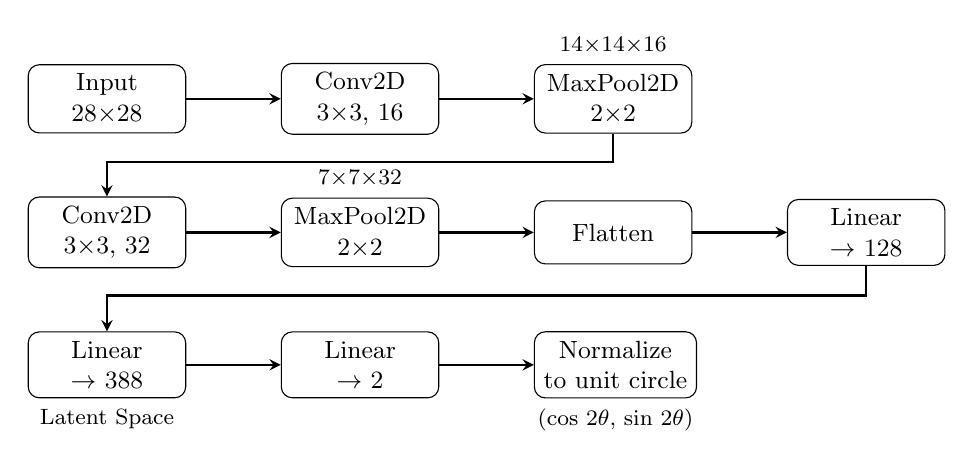
\begin{tikzpicture}[
        node distance=1.2cm,
        box/.style={
            rectangle,
            draw,
            minimum width=2cm,
            minimum height=0.8cm,
            align=center,
            rounded corners,
            font=\small
        },
        arrow/.style={
            ->,
            thick,
            >=stealth
        }
    ]

    % Input layer
    \node[box] (input) {Input\\28$\times$28};

    % First conv block
    \node[box, right=of input] (conv1) {Conv2D\\3$\times$3, 16};
    \node[box, right=of conv1] (pool1) {MaxPool2D\\2$\times$2};

    % Second conv block
    \node[box, below=0.8cm of input] (conv2) {Conv2D\\3$\times$3, 32};
    \node[box, right=of conv2] (pool2) {MaxPool2D\\2$\times$2};

    % Flatten and FC layers
    \node[box, right=of pool2] (flatten) {Flatten};
    \node[box, right=of flatten] (fc1) {Linear\\$\rightarrow$ 128};
    
    % Second row of FC layers
    \node[box, below=0.8cm of conv2] (fc2) {Linear\\$\rightarrow$ 388};
    \node[box, right=of fc2] (output_raw) {Linear\\$\rightarrow$ 2};
    \node[box, right=of output_raw] (output_norm) {Normalize\\to unit circle};

    % Connections - modified to create column-like flow
    \draw[arrow] (input) -- (conv1);
    \draw[arrow] (conv1) -- (pool1);
    
    % Modified connections to go down and then across instead of diagonal
    \draw[arrow] (pool1) -- ++(0,-0.8cm) -| (conv2);
    \draw[arrow] (conv2) -- (pool2);
    \draw[arrow] (pool2) -- (flatten);
    \draw[arrow] (flatten) -- (fc1);
    
    % Modified connection to go down and then across
    \draw[arrow] (fc1) -- ++(0,-0.8cm) -| (fc2);
    \draw[arrow] (fc2) -- (output_raw);
    \draw[arrow] (output_raw) -- (output_norm);

    % Add dimensions as labels
    \node[above=0.01cm of pool1, font=\footnotesize] {14$\times$14$\times$16};
    \node[above=0.01cm of pool2, font=\footnotesize] {7$\times$7$\times$32};
    \node[below=0.01cm of fc2, font=\footnotesize] {Latent Space};
    \node[below=0.01cm of output_norm, font=\footnotesize] {(cos $2\theta$, sin $2\theta$)};

    \end{tikzpicture}
    \caption{Neural network architecture used for the ANN circular manifold experiment. The network processes grating stimuli through convolutional layers, followed by fully connected layers that produce a 388-dimensional latent space. The output layer predicts raw values that are then normalized to the unit circle to represent the cosine and sine of the orientation angle.}
    \label{fig:nn}
\end{figure}

After training, we extracted the 388-dimensional latent representations for test stimuli and perfomed PCA to visualize the structure of these representations. The results revealed a striking circular manifold in the latent space, where stimuli with similar orientations were positioned close together, and the entire orientation space was represented as a continuous ring.

This circular topology emerged naturally from the training process, despite no explicit topological constraints being imposed on the network (Fig.~\ref{fig:manifold_analysis}). Through backpropagation, the network discovered that a circular representation is the most efficient way to encode a periodic variable, demonstrating how the geometry of the task space (in this case, the circular nature of orientation angles) becomes reflected in the geometry of the artificial neural representations.

\begin{figure}[h!]
    \centering
    \begin{subfigure}[b]{0.48\textwidth}
        \centering
        \includegraphics[width=\textwidth]{results/ann_circular_colormap_visualization.pdf}
        % \caption{Circular colormap visualization of the latent space, showing how orientation angles map onto the manifold. Note the overlapping of orientations 180\textdegree apart.}
        \label{fig:circular_colormap}
    \end{subfigure}
    \hfill
    \begin{subfigure}[b]{0.48\textwidth}
        \centering
        \includegraphics[width=\textwidth]{results/ann_circular_regression.pdf}
        % \caption{Circular regression analysis demonstrating the relationship between true orientation angles and their position on the manifold.}
        \label{fig:circular_regression}
    \end{subfigure}
    \caption{Analysis of the circular manifold in the CNN's latent space. Left, circular colormap visualization of the latent space, showing how orientation angles map onto the manifold. Note the overlapping of orientations 180\textdegree apart and the directional flow. Right, circular regression (fit   a model of the form $y = a\cos(2\theta) + b\sin(2\theta) + c$) analysis demonstrating the relationship between true orientation angles and their position on the PCA-derived manifold.}
    \label{fig:manifold_analysis}
\end{figure}

The experiment highlights several key principles of neural population geometry. First, the network's internal representations form a low-dimensional manifold (a circle) embedded in the high-dimensional latent space. Second, the topology of the manifold (circular) matches the topology of the task space (orientation angles), demonstrating topological correspondence. Third, similar stimuli are mapped to nearby points on the manifold, preserving the continuity of the input space through continuous representation. Finally, the network learns to compress the high-dimensional input (grating images) into a low-dimensional representation that captures the essential variable (orientation), effectively performing dimensionality reduction.

This simple experiment provides an intuitive foundation for understanding how more complex neural networks might represent more complicated manifolds in their latent spaces, and how the geometry of these representations relates to the computational tasks being performed.

\section{Neural geometry of a biological neural circuit}

After discovering a circular manifold in our artificial neural network, we investigated whether this topological structure exists in biological networks. We recorded activity from hundreds of neurons in an awake mouse's visual cortex while presenting the same grating stimuli shown in Fig. \ref{fig:grating_samples}, enabling direct comparison between artificial and biological neural representations.

\subsection{Neural recordings}

We performed 2-photon imaging to measure single-cell visual responses in the primary visual cortex (V1) of awake, head-fixed transgenic mice expressing the calcium indicator GCaMP6s in excitatory neurons (Fig. \ref{fig:technique.jpg}, A). GCaMP6s works as a fluorescent calcium sensor that responds to action potentials. When a neuron activates, calcium floods in, binding to the GCaMP protein and causing it to fluoresce brighter. By imaging this fluorescence change, we can track which neurons are active and when. GCaMP6s specifically offers high sensitivity (can detect single action potentials), making it ideal for capturing neural activity patterns. 

We recorded mouse V1 responses to 18 drifting gratings (spanning 0-360 degrees), each presented 10 times in pseudo-random order. Gratings stimuli were made of bars with spatial frequence 0.04 cpd while the drifting frequency was 2Hz. Each trial (180 total) consisted of 2 seconds blank screen followed by 2 seconds stimulus presentation. Neural activity was captured at 10Hz using two-photon imaging, with traces extracted via Suite2p \cite{pachitariu2016suite2p} . 

\begin{figure}[h!]
    \centering
    \includegraphics[width=\linewidth]{results/technique.jpg}
    \caption{\textbf{Experimental set-up}. \textbf{A}: schematic of experiment: the mice is head-fixed while passively viewing gratings of different orientations. \textbf{B} Left: image of the entirety of the cranial window, primary visual cortex corresponds to the largest blue region, while other visual areas are around it. Right: Raw image of the field of view of the two-photon microscope. The green circles correspond to active single neurons.} 
    \label{fig:technique.jpg}
\end{figure}

\subsection{Orientation tuning analysis}

Hubel and Wiesel's pioneering work demonstrated that V1 neurons respond selectively to edges of specific orientations \cite{hubel1959receptive}. This orientation selectivity forms the foundation of edge detection in the visual system, allowing the brain to extract critical contour information from complex scenes. This neural mechanism is essential for segmenting visual input into coherent objects and backgrounds, facilitating higher-level processes of object recognition and scene understanding. Therefore, a first step towards exploring how the population encodes orientation we must understand how single cells are tuned to different orientations.

To analyze orientation tuning, we quantified neural responses as normalized fluorescence changes:

$$\frac{\Delta F}{F} = \frac{F(t) - F_0}{F_0}$$

where $F(t)$ is fluorescence at time $t$ and $F_0$ is baseline fluorescence. Figure \ref{fig:analysis.jpg}A shows three neurons responding selectively to specific orientations. We calculated mean responses across trials for each orientation and fitted these with double Gaussians to extract tuning properties.

Orientation and direction selectivity were quantified using:

$$\text{OSI} = \frac{R_{\text{pref}} - R_{\text{orth}}}{R_{\text{pref}} + R_{\text{orth}}} \quad \text{and} \quad \text{DSI} = \frac{R_{\text{pref}} - R_{\text{opp}}}{R_{\text{pref}} + R_{\text{opp}}}$$

where OSI compares responses at preferred vs. orthogonal orientations, and DSI compares responses to preferred vs. opposite directions. \\

\begin{figure}[h!] 
    \centering
    \includegraphics[width=\linewidth]{results/analysis-figure.jpg}
    \caption{\textbf{Experimental set-up}. \textbf{A}: Raw responses to visual stimulus. \textbf{B}: For the same three neurons, every row shows their response to orientations. Blue dots are the mean response to each orientation. Red curve is the double gaussian fit. Box shows the parameters of the fit. \textbf{C}: population tuning distributions. Top: preferred orientation. Middle: OSI, Bottom: DSI} 
    \label{fig:analysis.jpg}
\end{figure}

Figure \ref{fig:analysis.jpg} illustrates our neuronal population's tuning properties. Neurons responded to all orientations with non-uniform distribution, with most cells showing direction selectivity ($DSI\geq0.5$). While neurons typically respond to both preferred and opposite orientations, responses are generally stronger at one peak (Fig \ref{fig:analysis.jpg}B, firs two neurons). In summary, this analysis reveals single-neuron tuning properties but it doesn't capture population-level orientation coding or potential emergent topological structures in the collective neural response patterns.

\subsection{Topology of neural responses}

First, to study if any emergent signature emerged from the neural population, we performed PCA to reduce the neural space of the 388 neurons to visualize the structure of the representation. Similarly as in Figure \ref{fig:manifold_analysis}, we see in Figure \ref{fig:mouse_manifold_analysis} that in the latent space a circular-like pattern emerges. The transition dynamics between orientations also show that similar orientations tend to be represented closer in the latent space. It is worth noting that no manipulations or assumptions about the neural data were made. 

\begin{figure}[h!]
    \centering
    \begin{subfigure}[b]{0.48\textwidth}
        \centering
        \includegraphics[width=\textwidth]{results/mouse_circular_colormap_visualization.pdf}
     
        \label{fig:mouse_colormap}
    \end{subfigure}
    \hfill
    \begin{subfigure}[b]{0.48\textwidth}
        \centering
        \includegraphics[width=\textwidth]{results/mouse_circular_regression.pdf}

        \label{fig:mouse_regression}
    \end{subfigure}
        \caption{Analysis of the circular manifold in the neuronal state space. Left, circular colormap visualization of the space, showing how orientation angles map onto the manifold. Note the near overlapping of orientations 180\textdegree apart and the directional flow. Right, circular regression (fit   a model of the form $y = a\cos(2\theta) + b\sin(2\theta) + c$) analysis demonstrating the relationship between true orientation angles and their position on the PCA-derived manifold.}
    \label{fig:mouse_manifold_analysis}
\end{figure}

To study in more detail the topological signature of the neural data, we proceeded to perform a persistent homology analysis of the latent space. This approach tracks topological features (loops, cavities) that persist across different scales, allowing us to identify the underlying manifold structure. By examining which features remain stable through multiple scales, we can distinguish between different manifold types (such as circles, tori, or spheres) without making prior assumptions about the neural data structure.

Although dimensionality reduction via PCA proved useful to show the circle-like structure, it assumes that the underlying structure of the data is linear. Visual cortex neurons show significant nonlinearities, including contrast saturation, phase invariance and surround suppression \cite{david2004natural}. Therefore, to study the topology of the neural manifold in latent space, non-linear dimensionality reduction techniques are more appropriate. The topology analysis thefore employed Uniform Manifold Approximation and Projection (UMAP) due to its superior ability to preserve local neighborhood structures. The projection of the first two dimensions of UMAP dimensionality reduction to the neural data can be seen in \ref{fig:topology.jpg}A.

\begin{figure}[h!]
    \centering
    \includegraphics[width=\linewidth]{results/topolgy.jpg}
    \caption{\textbf{Topology analysis}. \textbf{A}: Latent space shown in the first 2 dimensions \textbf{B}: Persistence diagram. \textbf{C}: Persistence barcode} 
    \label{fig:topology.jpg}
\end{figure}

Figure \ref{fig:topology.jpg} B-C presents the persistent homology analysis results. Figure \ref{fig:topology.jpg}B reveals a significant 1-dimensional homological feature ($H_{1}$) that emerges early and persists across multiple filtration radii, indicating a robust circular structure. The persistence barcode in Fig \ref{fig:topology.jpg}C quantifies this topological invariant, displaying a single dominant 1-dimensional homology class with extended persistence. This singular persistent $H_{1}$ feature provides strong evidence that the neural manifold forms a topologically circular structure.

In this biological network, the topological signature observed in the latent space reflects the structure of visual input arriving at the visual system, rather than intrinsic connectivity patterns. Orientation-tuned responses originate in the visual thalamus, which processes retinal input before broadcasting orientation information to primary visual cortex. The emergence of a circular signature should not be attributed to connectivity dynamics within the visual cortex itself—unlike the head direction system, which requires specific connectivity to maintain its ring attractor dynamics. Nevertheless, population geometry analysis revealed aspects of visual stimulus representation in the cortex that single-neuron analyses failed to capture.

\section{Conclusion}

In this technical report, we have presented neural population geometry as a unified framework for analyzing representations in both biological and artificial neural systems. Through illustrative examples from ANN simulation and neural recording from mouse visual cortex, we demonstrated how this geometric approach reveals insights about information encoding that traditional single-neuron analyses might miss.

First, the representation of neural activity as points in a high-dimensional state space, where each dimension corresponds to a single neuron's activity. We showed how these representations form structured manifolds with specific geometric and topological properties. Moreover, these manifolds develop a ring-shaped structure that preserve the circular nature of orientation space

Second, the utility of dimensionality reduction and geometric analysis techniques for visualizing and quantifying these neural manifolds. These methods allow us to extract meaningful structure from high-dimensional neural data and relate it to the computational task being performed.

The parallel analysis of biological and artificial systems illustrates how neural population geometry provides a common language for understanding information processing across different types of neural architectures. This approach bridges neuroscience and machine learning, offering tools for interpreting neural dynamics in both fields.

As recording technologies continue to advance, enabling simultaneous recordings from even larger neural populations, geometric approaches will become increasingly important for extracting meaningful patterns from high-dimensional neural data. Similarly, as artificial neural networks grow in complexity, analyzing their latent representations using geometric methods may provide insights into how they solve computational problems.

Although they have proven exceptionally useful, the interpretation of neural manifolds requires caution. While they successfully predict connectivity in specific cases (like the fly's central complex connectivity \cite{kim2017ring}), manifold emergence doesn't necessarily indicate connectivity or dynamic patterns. In mouse visual cortex, the orientation manifold described in this report reflects input structure rather than neural connectivity.
Additionally, dimensionality reduction methods essential to these analyses introduce their own limitations. UMAP, for example, captures local topological features but may misrepresent global geometric structures, long-range relationships, and broader patterns. \cite{diaz2021review}

In summary, this report demonstrates that neural population geometry offers a powerful conceptual framework and analytical toolkit for understanding neural computation across biological and artificial systems.
\bibliographystyle{unsrt}
\bibliography{refs}

\end{document}
